\section{Permutations}
Ladder lotteries and permutations are intricately related to each other. 
The research for The Canonical Ladder Listing Problem is highly influenced 
by permutation listing algorithms. Knuth describes a number of 
permutation listing algorithms in \emph{The Art of Computer Programming}~\cite{A18}. During the research for The Canonical Ladder Listing Problem, twelve of these 
enumeration algorithms were investigated~\cite{A18,A19,A20,A24,A25,A26,A31,A34,A35,A36,A37}.\par 
We define \emph{$S_{n}$} as the set of all $n!$ permutations of order $n$. 
The first algorithm we looked at for listing $S_{n}$ is the lexicographic algorithm, which orders all $n!$ permutations from smallest to largest. The lexicographic 
algorithm generates each permutation with an amortized time of $O(n^{2}log(n))$~\cite{A20}. The second of which is the 
colexicographic algorithm which orders all $n!$ permutations from largest to smallest. The colexicographic 
algorithm generates each permutation with an amortized time of $O(n^{2}log(n))$~\cite{A19}. The third of which is Zak's 
algorithm which lists $S_{n}$ by reversing a suffix in one permutation to get to the next 
permutation. The time complexity of Zak's algorithm constant amortized time~\cite{A31}.
The fourth of which is Heap's algorithm which is a decrease and conquer algorithm.  
The time complexity of Heap's algorithm is {\sc CAT}, constant amortized time of $O(1)$ per permutation~\cite{A24}.
The fifth algorithm is the Steinhaus-Johnson-Trotter (SJT) algorithm which generates $S_{n}$ by performing adjacent swap operations 
on the permutation resulting in the next permutation. Thus, each permutation in $S_{n}$ differs 
from it predecessor by a single swap operation, making SJT a Gray code~\cite{A25}. To go from any two successive permutations, 
the time complexity is $O(1)$~\cite{A25}.
The sixth algorithm is the algorithm using star transpositions that always swaps the first element of the permutation 
with some other element. It was discovered by Gideon Ehrlich and is described as Algorithm E in Knuth's book~\cite{A18}.
The seventh algorithm is the derangement ordering in which no two consecutive permutations have any elements 
in the same position. It was first discussed by Savage in~\cite{A35}. 
The eighth algorithm is the Single Track listing algorithm. Each column in the list of permutations 
is a cyclic shift of the first column~\cite{A36}. The computation for each successive permutation 
is CAT~\cite{A36}.
The ninth algorithm is the Single Track Gray Code listing algorithm. The properties of the Single Track 
listing algorithm hold. Furthermore, any two successive permutations differing by at most two transpositions~\cite{A36}.
The tenth listing algorithm is found in Knuth's book. At each step, it either rotates the permutation to the left by one 
or swaps the first two elements~\cite{A37}. The problem as to whether such a listing algorithm exists for all $n$ 
is posed as an open problem in Knuth's book~\cite{A37}. It was solved by Sawada and Williams in their paper 
\emph{A Hamiltonian Path for the Sigma-Tau Problem}~\cite{A38}.
The eleventh algorithm is Corbett's algorithm which rotates a prefix of the first possible length in 
$n$,$2$,$n-1$,$3$,$n-2$,$4$, etc.~\cite{A34}. 
% The twelfth algorithm is Effler and Ruskey's algorithm which lists permutations by groups of $k$ inversions. %Their algorithm has 
% constant amortized time algorithm for generating permutations of order $n$ with $k$ inversions~\cite{A26} meaning 
%the time it takes to generate each permutation is bounded by a constant.
%The algorithm is also a \emph{BEST} algorithm (backtracking ensures success at terminals), meaning that when the algorithm backtracks, 
%the back-tracking leads to a successful result~\cite{A26}. 
To see the listings for all the aforementioned algorithms, refer to Figure~\ref{Fig:11perms}\cite{A42}.\par
\begin{figure} 
    \centering 
    \resizebox{.65\textwidth}{.3\textheight}{
            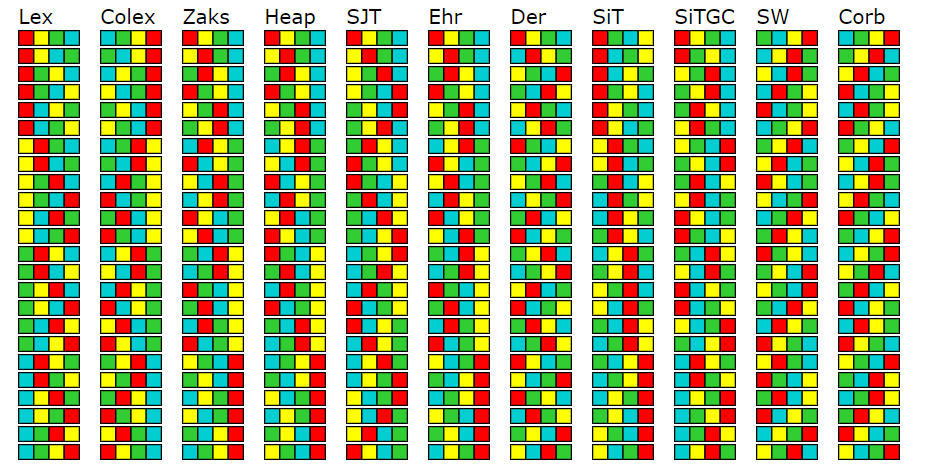
\includegraphics{11perms}
    }
    \caption{Eleven permutation listing algorithms}
    \label{Fig:11perms}
\end{figure}

In Chapter 1, it was stated that a modification of the SJT algorithm was used to solve The Canonical Ladder Listing Problem. 
SJT generates each permutation in $O(1)$ per permutation and in Gray code order. In Chapter 4, the SJT 
algorithm is modified to create ladders instead of permutations while still maintaining the same efficiency and order. 
Below, we further examine the SJT algorithm.

%Paragraph SJT
\subsection{Steinhaus-Johnson-Trotter Algorithm}
The Steinhaus-Johnson-Trotter algorithm generates $S_{n}$ by performing adjacent swap operations 
on the permutation resulting in the next permutation. Thus, each permutation in $S_{n}$ differs 
from it predecessor by a single swap operation. Let an \emph{even permutation} be defined as a permutation 
with an even number of inversions. Let an \emph{odd permutation} be defined as a 
permutation with an odd number of inversions. If $\pi$ of order $n-1$ is an even permutation, then the $nth$ element is inserted into all 
positions of $\pi$ of order $n-1$ in descending order. 
If $\pi$ of order $n-1$ is an odd permutation, the $nth$ element is inserted into all positions of $\pi$ of order $n-1$ in ascending order~\cite{A25}. 
For $\pi$ of order $1$ we have $\pi=(1)$. Since 
there are no inversions in $\pi=(1)$ it is even. Now insert $2$ in all positions in $\pi=(1)$
in descending order. Thus we get $(1,2)$ followed by $(2,1)$. Since $(1,2)$ is 
an even permutation, insert $3$ into all positions in descending order resulting in $(1,2,3)$,
$(1,3,2)$ and $(3,1,2)$. Since $(2,1)$ is an odd permutation, insert $3$ 
into all permutations in ascending order resulting in $(3,2,1)$, $(2,3,1)$ and $(2,1,3)$.\par 
% Initialize $\pi$ to the identity permutation, initialize $currentElement$ to $2$, initialize 
% $n$ to $p_{max}$. Let $direction$ be a Boolean array of size $n$ initialized to $true/right$ for all indices. 
% If $currentElement$ is greater than $n$, print $\pi$ 
% and return. Otherwise, begin a for loop that runs $i=[1 \dots n-1]$ times. 
% In the for loop, first make a recursive call with $currentElement$ increasing by one. 
% If $direction[currentElement]$ is $right$, then swap $currentElement$ in $\pi$ with its left neighbor. Else 
% if $direction[currentElement]$ is $left$ then swap the $currentElement$ in $\pi$ with its right neighbor.
% Once the for loop has exited, make one more recursive call with $currentElement+1$ outside the for loop; 
% this avoids an extra swap operation from occurring while still maintaining the correct number of recursive 
% calls. Lastly, negate $direction[currentElement]$, which effectively changes the direction of the $currentElement$ to be swapped.
% To see the Steinhaus-Johnson-Trotter algorithm please refer to Algorithm~\ref{Alg:SJT}.

% \begin{algorithm}
%     \begin{algorithmic}[1]
%         \Function{SJT}{$\pi$, $currentElement$, $n$, $direction$}
%             \If{$currentElement > n$}
%                 \If{{\sc Sorted($\pi$)}}
%                     \State {\sc Print($\pi$)}
%                 \EndIf
%                 \State \textbf{return}
%             \EndIf
%             \For{$i$ \textbf{from} $1$ \textbf{to} $currentElement-1$}
%                 \State {\sc SJT($\pi$, $currentElement+1$, $n$)}
%                 \State $index \gets $ index of $currentElement$ in $\pi$
%                 \If{$direction[currentElement]=right$}
%                     \State {\sc Swap}$(p_{index}, p_{index-1})$
%                 \Else 
%                     \State {\sc Swap}$(p_{index}, p_{index+1})$
%                 \EndIf
%                 \State {\sc Print}$(\pi)$
%             \EndFor
%             \State {\sc SJT}($\pi$, $currentElement+1$, $n$, $direction$)
%             \If{$direction[currentElement]=right$}
%                 \State $direction[currentElement] \gets left$
%             \Else 
%                 \State $direction[currentElement] \gets right$
%             \EndIf
%         \EndFunction
        
%     \end{algorithmic}
%     \caption{SJT Algorithm for listing $S_{n}$}
%     \label{Alg:SJT}
% \end{algorithm}

The Steinhaus-Johnson-Trotter algorithm is a Gray code, meaning that in order to transition 
between any two subsequent permutations in $S_{n}$, there is a minimal amount of constant 
change required. The algorithm simply swaps two elements in order to transition between 
permutations. Each recursive call creates a new permutation with the exception of the 
initial call to the function in which $n$ recursive calls need to be made before the 
first permutation is printed. The amortized time to transition between permutations is $O(1)$.





